
% Works
% -----

\subsection{Conditional Operation and Inverse Sequences}

\begin{mydef}[Sets of sequences]
As we will frequently refer to sets of fequences,
we will use calligraphic letters (e.g. $\sqs{A}$, $\sqs{B}$, $\sqs{C}$ and $\sqs{S}$)
to denote such sets for brevity.
We will use $A\cc\sqs{B}$ to denote the set of sequences $\{A\cc B|B\in\sqs{B}\}$,
and $\Dom{\sqs{A}}$ to denote $\bigcap_{A\in\sqs{A}} \Dom{A}$.
\end{mydef}

% works operators
% ---------------

\begin{mydef}[$\worksmsign$, $\worksmeqsign$]
For two sets of sequences $\sqs{A}$ and $\sqs{B}$
we write $\worksm{\sqs{A}}{\sqs{B}}$ iff $\Dom{\sqs{A}} \subseteq \Dom{\sqs{B}}$;
that is, if all sequences in $\sqs{B}$ work (do not break the filesystem)
on any filesystem all sequences in $\sqs{A}$ work on.
We write $\worksmstr{\sqs{A}}{\sqs{B}}$ iff $\Dom{\sqs{A}} \subset \Dom{\sqs{B}}$.

As a special case, we write $\worksmnil{\sqs{A}}$ if we know that there is a filesystem
all sequences in $\sqs{A}$ work on.
We also apply these relations to sequences directly:
$\worksm{A}{B}$ with the meaning $\worksm{\{A\}}{\{B\}}$.
\end{mydef}

In a sense, $A\worksmeqsign B$ is a weaker counterpart of $A\eqext B$, as the former
only requires that $B$ works where $A$ works, where the latter also requires
that their effect is the same.
It is easy to see that the following corollaries are true:

\begin{mycor}\label{worksextpostfix}
% An inference rule in the algebra
$\forall A,S: \worksm{A\cc S}{A}$, that is, if a sequence works, its initial segment also works.
\end{mycor}

\begin{mycor}\label{workschained}
% An inference rule in the algebra
$\worksmeqsign$ can be chained:
if $\sqs{B'}\subseteq\sqs{B}$, then
$\worksm{\sqs{A}}{\sqs{B}} \wedge \worksm{\sqs{B'}}{\sqs{C}} \Rightarrow \worksm{\sqs{A}}{\sqs{B}\cup\sqs{C}}$.
\end{mycor}

We also prove the following lemmas.

\begin{myax}\label{combine_independent_commands}
The combination of independent commands works wherever the original commands work:
\[ \alpha\indep \beta \Rightarrow \worksm{\{\alpha, \beta\}}{\{\alpha\cc \beta\}}. \]
\end{myax}
\begin{proof}
We name this proposition a \namecref{combine_independent_commands} 
because to prove it, we must reach back to our filesystem model.
Let $\alpha=\cxynv$ and $\beta=\czwmv$.
We prove the proposition by contradiction and
assume that there is a filesystem $\FS$ for which
$\cxynv\aFS\neq\fsbroken$ and $\czwmv\aFS\neq\fsbroken$, but
$\cxynv\cc \czwmv\aFS=\fsbroken$.
We know $\cxynv\aFS\neq\fsbroken$ so it must be applying 
$\czwmv$ that breaks it.
Applying a command can only result in a broken filesystem in two cases.
First, if the input type does not match the filesystem,
but we know $[\FS(m)]=[w]$ and so
$[(\cxynv\aFS)(m)]=[w]$ as based on \cref{incomparable_is_independent}, $n\neq m$.
Second, if the new filesystem violates the tree property.
This again cannot be the case because we also know that $n\unrel m$
and the tree property only depends on the types of values at the parent and children of $m$,
which therefore cannot be changed by $\cxynv$.
\end{proof}

This result can be extended to sequences:

\begin{mylem}\label{combine_independent_sequences}
The combination of independent sequences works wherever the original sequences work:
\[ S\indep T \Rightarrow \worksm{\{S,T\}}{\{S\cc T\}}. \]
\end{mylem}
\begin{proof}
Assume that there is a filesystem $\FS$ so that
$S\aFS\neq\fsbroken$ and $T\aFS\neq\fsbroken$, but
$(S\cc T)\FS=\fsbroken$.

From \cref{def_indep} we know that
the commands in $S$ and $T$ pairwise commute, and so any sequence
that contains the commands from $S$ and $T$ and preserve their original partial order
is equivalent to $S\cc T$ on all filesystems.

Let the command that breaks $\FS$ in $T$ when applying $S\cc T$ be $t$
so that $T=T_0\cc t\cc T_1$.
It is still true that $(T_0 \cc t)\FS\neq\fsbroken$,
and by definition $(S\cc T_0)\FS\neq\fsbroken$,
but $(S\cc T_0\cc t)\FS=\fsbroken$.
Also, from above we know that $S\cc T_0\equiv T_0\cc S$
and so $(T_0 \cc S)\FS\neq\fsbroken$.

If we denote the first command in $S$ with $s_1$,
this means that $(T_0 \cc s_1)\FS\neq\fsbroken$,
which we can combine with $(T_0 \cc t)\FS\neq\fsbroken$, $t\indep s_1$ and
\cref{combine_independent_commands}
(using $T_0\FS$ as the reference filesystem)
to arrive at $(T_0 \cc s_1\cc t)\FS\neq\fsbroken$.

We can repeat this step for $s_2$, the next command in $S$,
and from 
$(T_0 \cc s_1\cc t)\FS\neq\fsbroken$
and
$(T_0 \cc s_1\cc s_2)\FS\neq\fsbroken$
arrive at
$(T_0 \cc s_1\cc s_2\cc t)\FS\neq\fsbroken$.
This can be repeated until $S$ is exhausted and we get
$(T_0 \cc S\cc t)\FS\neq\fsbroken$, which is a contradiction.
\end{proof}

We also prove the following:

\begin{mylem}\label{worksinputmatch}
If $A$ and $B$ are minimal sequences, $\worksmnil{\{A,B\}}$,
and there are commands on node $n$ in both $A$ ($\cxynv\in A$) and $B$ ($\czwnv\in B$),
then the input types of these commands must match ($[x]=[z]$).
\end{mylem}
\begin{proof}
This result is similar to \cref{equiv_simple_same_commands} and
is easily shown using a proof by contradiction: if $[x]\neq [z]$, then there is no filesystem that
either $\cxynv$ or $\czwnv$ would not break, 
and consequently $A$ and $B$ cannot work on the same filesystem.
\end{proof}


\bigskip

% Type equivalence classes
% ------------------------

\noindent
For the proof of the correctness of the reconciliation algorithm,
we will also need a way of moving parts of sequences between the two
sides of the $\worksmeqsign$ relation.
We can do this based on the observation that commands are bijections
if we only distinguish between types in our objects.
To formalise this, we extend type equality ($\typeeq$)
to filesystems, commands and sequences of commands.
\begin{mydef}[Equivalence by type, extended: $\typeeq$]
$ $ % otherwise first list element starts on same line
\begin{itemize}
\item For two filesystems $\FS\typeeq\GS$ iff they share the same nodes $\setn$,
and for all $n\in\setn$, $\FS(n) \typeeq \GS(n)$.
\item For two commands $\cxynv\typeeq\czwmv$ iff 
$x\typeeq z$ and $y\typeeq w$
(that is, $[x]=[z]$ and $[y]=[w]$)
and $n=m$.
\item For two sequences of commands $\emptyseq\typeeq\emptyseq$, and
if $A'=\alpha\cc A$ and $B'=\beta\cc B$, then $A'\typeeq B'$ iff $\alpha\typeeq\beta$ and $A\typeeq B$.
\end{itemize}
\end{mydef}

We select representatives of each $\typeeq$-equivalence class of values:
for $[\empt]$ and $[\vald]$ this must be $\empt$ and $\vald$; and
for $[\valf]$ we select an arbitrary file value $\fil\in[\valf]$.
We then use these representative values to
introduce the canonical mapping $\T$ that preserves the types of values,
but maps all objects into a subsystem where there is a one-to-one
correspondence between types and values.

\begin{mydef}[$\T$]
We use $\T$ and write $a\T$ to denote the canonical mapping of 
values, filesystems, commands and sequences to the
representatives of their $\typeeq$-equivalence class.
\begin{itemize}
\item For values, $\vald\T=\vald$, $\valf\T=\fil$ and $\empt\T=\empt$.
\item For filesystems, $\FS\T$ is defined by $\FS\T(n) = \FS(n)\T$.
\item For commands, $\cbrk\T=\cbrk$ and $\cxynv\T = \cTxynv$.
\item For sequences of commands, $\emptyseq\T=\emptyseq$, and if $S'=\alpha\cc S$, then $S'\T=\alpha\T\cc S\T$.
\item Finally we extend $\T$ to sets of sequences: $\sqs{A}\T = \{S\T | S\in\sqs{A}\}$.
\end{itemize}
\end{mydef}

It is easy to see that for all objects where it is defined, $a\T\typeeq a$.
% $|\setf|$ is also $1$.
As representatives of filesystems, commands, sequences, etc.
are subsets of their non-representative counterparts, all
propositions proven so far apply to them as well.

\begin{mycor}
For any filesystem $\FS$ and command $\alpha$, 
$\alpha\T(\FS\T) = (\alpha\aFS)\T$.
TODO needed?
\end{mycor}

% It is easy to see that 
% $A\equiv B \Rightarrow A\T\equiv B\T$ 
% and
% $A\eqext B \Rightarrow A\T\eqext B\T$,
% but the reverse is not true as 
% $A\T$ and $B\T$ will have the same effect on all filesystems
% if $A$ and $B$ differ only in some of the values in their commands,
% whereas clearly $A\nequiv B$.

As the types of values determine whether a command breaks a filesystem,
we know $\Dom{A}=\Dom{A\T}$ and therefore $\Dom{\sqs{A}}=\Dom{\sqs{A}\T}$.
From this it follows that

\begin{mycor}\label{repr_works_is_same}
\begin{gather*}
\worksmnil{\sqs{A}} \Longleftrightarrow \worksmnil{\sqs{A}\T} \\
\worksm{\sqs{A}}{\sqs{B}} \Longleftrightarrow \worksm{\sqs{A}\T}{\sqs{B}\T}.
\end{gather*}
\end{mycor}

% Inverse commands
% ----------------

We are now ready to define the inverse of representative commands $\alpha\T$
which allows us to move parts of sequences between the
two sides of $\worksmeqsign$.
This is based on the following observation.

\begin{mylem}\label{repr_comm_inject}
Representative commands $\alpha\T$ are partial bijections over representative filesystems ($\FS\T$).
Because partial functions are trivially surjective when restricted to their images, this is
equivalent to saying that representative functions are injective except for cases
where they break a filesystem (they are not defined):
\[ \forall\FS,\GS,\alpha: \FS\T\neq\GS\T \wedge \alpha\T(\FS\T)\neq\fsbroken \Longrightarrow \alpha\T(\FS\T) \neq \alpha\T(\GS\T). \]
\end{mylem}
\begin{proof}
This is trivial if $\GS\T=\fsbroken$, so we assume it is not so.
Let $\alpha\T = \cTxynv$.
If $\FS\T$ and $\GS\T$ have different values at any node apart from $n$, then this difference remains
even after applying $\cTxynv$ to $\FS\T$. The only remaining case therefore is where they have the same values
at all nodes except $n$.
As $\cTxynv(\FS\T)\neq\fsbroken$, we know $[\FS\T(n)]=[x]$.
We also know that $\GS\T(n)\neq\FS\T(n)$, and therefore, as there is a one-to-one correspondence between values and types,
$[\GS\T(n)]\neq[x]$.
This implies $\cTxynv(\GS\T)=\fsbroken$,
and again we have $\alpha\T(\FS\T) \neq \alpha\T(\GS\T)$.
\end{proof}

% See
% https://en.wikipedia.org/wiki/Inverse_semigroup#Origins
% https://en.wikipedia.org/wiki/Symmetric_inverse_semigroup
% https://en.wikipedia.org/wiki/Partial_function

\begin{mydef}[Inverse commands and sequences]
We write $\alpha\T^{-1}$ for
the inverse of the representative command (partial bijection) $\alpha\T$.

We write ${S\T}^{-1}$ for the inverse of the sequence $S\T$, which consists of the inverses of the commands in $S\T$
in reverse order.
\end{mydef}
Per definition, for any filesystem $\FS\T$ outside the image of $\alpha\T$, the inverse $\alpha\T^{-1}$ is undefined.

\begin{mylem}
For representative commands
\[ \cTxynv^{-1} = \cTyxnv. \]
TODO needed? -maybe for \cref{negneg_is_typeeq}
\end{mylem}

From the definitions we can clearly see that
\begin{mycor}\label{negneg_is_typeeq}
$\forall S: ({S\T}^{-1})^{-1} = S\T$.
\end{mycor}

For brevity, in the following lemma we use $B$, $B'$, $\sqs{A}$ and $\sqs{C}$ to denote
representative sequences and sets.

\newcommand{\ia}{\sqs{A}}
\newcommand{\ic}{\sqs{C}}
\newcommand{\ibi}{B^{-1}}

\begin{mylem}\label{r_invmove}
A common initial segment of a set of \emph{representative} sequences can be moved 
to the other side of $\worksmeqsign$ by inverting it:
\begin{gather*}
\worksm{\ia}{B\cc\ic}
\ \Longleftrightarrow \ \worksm{\ibi\cc\ia}{\ic} 
\ \wedge \  \worksm{\ia}{\{B\}}
\end{gather*}
\end{mylem}
\begin{proof}
% This result is quite expected as we're mapping a subset statement using a bijection,
% but made more complicated a as B is not defined everywhere.

The proof is illustrated by \cref{fig_invmove}.

\begin{figure}[htb]
\begin{center}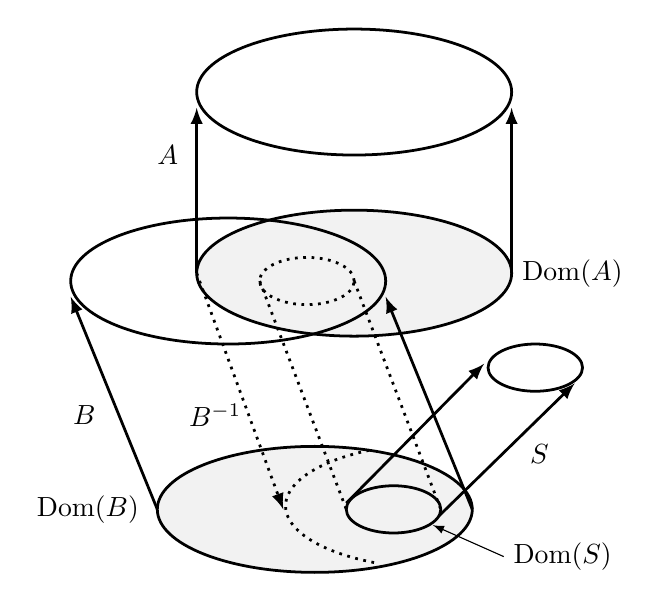
\begin{tikzpicture}
[line width=1pt]
\node at  (1.6+2, 0.1) [right] {$\textrm{Dom}(\seqset{A})$};
\draw[fill=black!5] (1.6, 0.1) ellipse (2cm and 0.8cm); %% Dom A
\draw               (1.6, 2.4) ellipse (2cm and 0.8cm); %% Img A
\draw[-latex] (1.6+2, 0.1)--(1.6+2, 2.4-.2); %% A right
\draw[-latex] (1.6-2, 0.1)--(1.6-2, 2.4-.2); %% A left
\node at  (1.6-2-.1, 1.6) [left] {$A$};
%%
\node at (1.1-2-.1, -2.9) [left] {$\textrm{Dom}(B)$};
\draw[fill=black!5] (1.1, -2.9) ellipse (2cm and 0.8cm); %% Dom B
\draw               (0  ,  0)   ellipse (2cm and 0.8cm); %% Img B
\draw[-latex] (1.1+2, -2.9)--(0+2, 0-.2); %% B right
\draw[-latex] (1.1-2, -2.9)--(0-2, 0-.2); %% B left
\node at  (0.55-2-.1, -1.7) [left] {$B$};
\draw[-latex,dotted] (1.6-2, 0.1)--(0.7, -2.9); %% B-1
\node at (0.3, -1.7) [left] {$B^{-1}$};
\draw[dotted] (1.79, -2.15) arc(118:244: 2cm and 0.8cm); %% Arc
\draw[dotted] (1, 0) ellipse (0.6cm and 0.3cm); %% Dotted S
\draw         (2.1, -2.9) ellipse (0.6cm and 0.3cm); %% Dom S
\draw[dotted] (1-0.6, 0)--(2.1-0.6, -2.9); %% B-1
\draw[dotted] (1+0.6, 0)--(2.1+0.6, -2.9); %% B-1
\draw                     (3.9, -1.1) ellipse (0.6cm and 0.3cm); %% Img S
\draw[-latex] (2.1-0.6, -2.9+.08)    --(3.9-0.6-.05, -1.1+.05); %% Left S
\draw[-latex] (2.1+0.6-.02, -2.9-.08)--(3.9+0.6-.1, -1.1-.2); %% Right S
\node at  (3.7,-2.2) [right] {$S$};
\draw[-latex,thin] (3.5, -3.5) node[right]{$\mathrm{Dom}(\seqset{S})$} -- (2.1+0.5, -2.9-0.2);
\end{tikzpicture}\end{center}

\caption{Proof of \cref{r_invmove}}\label{fig_invmove}
\end{figure}

Unless $\worksmnil{\ia}$, the propositions is trivially true. Otherwise,
for the left-to-right part of the proposition,
we know $\worksmnil{B\cc\ic}$, which implies that $\Dom{\ic}$ intersects with $\Img{B}$ 
as otherwise $B\cc\ic$ would break all filesystems.
As the (representative) $B$ is a bijection between its domain and image,
we can use $\ibi$ to map this intersection back
onto the domain of $B$ and get $\Dom{B\cc\ic}$.
As $\worksm{\ia}{B\cc\ic}$, 
we also know that $\Dom{\ia} \subseteq \Dom{B\cc\ic}$.
We now use $B$ to map both sides of this statement, which yields
$\Dom{B^{-1}\cc\ia} \subseteq \Dom{\ibi\cc B\cc\ic}$,
but the latter is a subset of $\Dom{\ic}$,
and so $\Dom{\ibi\cc\ia} \subseteq \Dom{\ic}$,
which is the same as $\worksm{\ibi\cc\ia}{\ic}$.

For the right-to-left part,
from $\worksm{\ia}{B}$ we know $\Dom{\ia} \subseteq \Dom{B}$.
Therefore we can project the whole of $\Dom{\ia}$ using the bijective representative sequence $B$
to get $\Dom{\ibi\cc\ia}$, and as $\worksm{\ibi\cc\ia}{\ic}$
we know
$\Dom{\ibi\cc\ia} \subseteq \Dom{\ic}$.
We use $\ibi$ to project both sides of this statement to get
$\Dom{B\cc\ibi\cc\ia} \subseteq \Dom{B\cc\ic}$.
But we also know that $\Dom{B\cc\ibi\cc\ia} = \Dom{\ia}$
as $\Dom{\ia} \subseteq \Dom{B}$,
and so $\Dom{\ia} \subseteq \Dom{B\cc\ic}$ which is the same as
$\worksm{\ia}{B\cc\ic}$.
\end{proof}


\begin{mylem}\label{indep_prefix_combine}
The combination of sequences with a common head and independent tails 
continues to work under the same conditions:
\[ \worksc{A\cc B}{\sqs{S}} \wedge \worksc{A\cc C}{\sqs{S}} \wedge B\indep C \Rightarrow \worksc{A\cc B\cc C}{\sqs{S}} \]
\end{mylem}
\begin{proof}
Based on \cref{repr_works_is_same} we have
$\worksc{A\T\cc B\T}{\sqs{S\T}}$ and $\worksc{A\T\cc C\T}{\sqs{S\T}}$,
and from \cref{r_invmove} we know
$\worksc{B\T}{{A\T}^{-1}\cc \sqs{S\T}}$ and $\worksc{C\T}{{A\T}^{-1}\cc \sqs{S\T}}$.
Using \cref{combine_independent_sequences} we get
$\worksc{B\T\cc C\T}{B\T,C\T}$,
and combining these using \cref{workschained}
we get
$\worksc{B\T\cc C\T}{{A\T}^{-1}\cc \sqs{S\T}}$.

From $\worksc{A\cc B}{\sqs{S}}$ we also know $\worksc{A}{\sqs{S}}$ and $\worksc{A\T}{\sqs{S\T}}$.
We can combine this and $\worksc{B\T\cc C\T}{{A\T}^{-1}\cc \sqs{S\T}}$ using
the second proposition of \cref{r_invmove} to get
$\worksc{A\T\cc B\T\cc C\T}{\sqs{S\T}}$, and from \cref{repr_works_is_same} we know
$\worksc{A\cc B\cc C}{\sqs{S}}$.
\end{proof}
